% This is "sig-alternate.tex" V2.0 May 2012
% This file should be compiled with V2.5 of "sig-alternate.cls" May 2012
%
% This example file demonstrates the use of the 'sig-alternate.cls'
% V2.5 LaTeX2e document class file. It is for those submitting
% articles to ACM Conference Proceedings WHO DO NOT WISH TO
% STRICTLY ADHERE TO THE SIGS (PUBS-BOARD-ENDORSED) STYLE.
% The 'sig-alternate.cls' file will produce a similar-looking,
% albeit, 'tighter' paper resulting in, invariably, fewer pages.
%
% ----------------------------------------------------------------------------------------------------------------
% This .tex file (and associated .cls V2.5) produces:
%       1) The Permission Statement
%       2) The Conference (location) Info information
%       3) The Copyright Line with ACM data
%       4) NO page numbers
%
% as against the acm_proc_article-sp.cls file which
% DOES NOT produce 1) thru' 3) above.
%
% Using 'sig-alternate.cls' you have control, however, from within
% the source .tex file, over both the CopyrightYear
% (defaulted to 200X) and the ACM Copyright Data
% (defaulted to X-XXXXX-XX-X/XX/XX).
% e.g.
% \CopyrightYear{2007} will cause 2007 to appear in the copyright line.
% \crdata{0-12345-67-8/90/12} will cause 0-12345-67-8/90/12 to appear in the copyright line.
%
% ---------------------------------------------------------------------------------------------------------------
% This .tex source is an example which *does* use
% the .bib file (from which the .bbl file % is produced).
% REMEMBER HOWEVER: After having produced the .bbl file,
% and prior to final submission, you *NEED* to 'insert'
% your .bbl file into your source .tex file so as to provide
% ONE 'self-contained' source file.
%
% ================= IF YOU HAVE QUESTIONS =======================
% Questions regarding the SIGS styles, SIGS policies and
% procedures, Conferences etc. should be sent to
% Adrienne Griscti (griscti@acm.org)
%
% Technical questions _only_ to
% Gerald Murray (murray@hq.acm.org)
% ===============================================================
%
% For tracking purposes - this is V2.0 - May 2012

\documentclass{sig-alternate}
\usepackage{graphicx}


\usepackage{blindtext}
\usepackage{url}
\usepackage{listings}
\usepackage{fancyvrb}
\usepackage{float}
\usepackage{hyperref}


\begin{document}
% % \degree{}
\title{BaseFS -\\ Basically Available, Soft State, Eventually Consistent Filesystem for Cluster Management}
\numberofauthors{1} %  in this sample file, there are a *total*
\author{
\alignauthor
Marc Aymerich Gubern\\
    \affaddr{Universitat Politecnica de Catalunya UPC}\\
    \email{marc.aymerich@est.fib.upc.edu}
}
\additionalauthors{}
\date{30 July 1999}

\maketitle

\begin{abstract}
BaseFS is a peer-to-peer distributed filesystem for cluster configuration, designed to operate under the harsh network conditions commonly found on Wireless Community Networks. Nodes do not need to trust each other, the core data-structure is an append-only 
% [EL] What is a DAG? write the full name the first time
Merkle DAG with monotonic and cryptographic properties that allows for efficient and secure verification of data sent by untrusted nodes. Decentralized write permission is achieve using a hierarchy-based public key infrastructure (PKI) built into the Merkle DAG, allowing for automatic resolution of write conflicts. Finally, a gossip layer is used for disseminate changes very quickly and efficiently as well as for maintaining cluster membership in an scalable way. With no single point-of-failure, BaseFS can provide levels of availability, scalability and performance never seen before on a cluster configuration tool.

\end{abstract}
% A category with the (minimum) three required fields
\section{Introduction}

One of the steps towards building a successful distributed system is establishing effective configuration management. It is a complex engineering process responsible for planning, identifying, tracking and verifying changes in the software and its configuration as well as maintaining configuration integrity throughout the life cycle of the system \cite{Yermolaiev:managing}.

todo the basic approach is to use a centralized database. orchestration

Some successful tools exist to aid in this process, e.g. Chef and Puppet only to name a few. In these solutions, the cluster configuration is written in recipes that converge every few minutes. While this approach works well for static configuration, it fails to provide an ideal solution for more dynamic state, where a near real-time convergence is desirable. Because of the need for faster provisioning (e.g. elasticity in cloud environments or quickly respond to failures) systems like Zookeeper, etcd or Consul have emerged that target this very specific problem. They are distributed key-value stores designed to keep the global state of the system. We can make a rough distinction between the \textit{static configuration management} tasks solved by tools like Chef or Puppet and the \textit{dynamic cluster management} commonly solved by K/V stores like Zookeeper, etcd or Consul.

Existing \textit{dynamic cluster management} solutions are designed with strong consistency models and client-server architectures. They have server nodes that require a quorum of nodes to operate (usually a simple majority). They choose consistency over availability under the face of a network partition. 
% [EL] ?? si la referencia va con la frase anterior, ponla antes del punto, y sino ponla al final de la frase
[2] These design decisions are based on the assumption that these systems are deployed on a datacenter-like environment, where machines are homogeneous, with predictable performance, connected by fast networks, with low churn and operated by a team of highly technical engineers, while all being part of a single administrative domain. But these assumptions are not always true.

Community cloud computing is an emerging model where infrastructure is built using a collaborative effort. It is often the result of individual users providing spare resources to a common pool. As we can imagine the set of constrains faced by this kind of distributed systems are different from those we can find in the typical datacenter. Hardware is heterogeneous, it tends to be consumer-grade with higher failure rates and lower performance. The network is slow and unreliable; partitions occur more often. Resources range in quantity and quality from one node to another. The administrative boundary between organizations is sometimes blurry, with requirements for a decentralized administration of the infrastructure. Limitations on the technical capacity for effectively deploying and managing complex distributed systems may also exist, since the operators are sometimes members of the community that volunteer their time, but with limited SLA commitment.

The main contribution of this thesis is to provide a novel approach to solve cluster configuration management problems on a decentralized, more networked constrain, environments. First we present a case for a more available and less consistent cluster management solution. Then, we introduce the design an implementation of BaseFS, an eventually consistent gossip-style distributed filesystem specifically designed for cluster and configuration management. Experimental results from a prototype implementation are presented in section \ref{evaluation}  and finally we reflect on the future of BaseFS.

\section{Background}

% [EL] Cada vez escribes key-value store de una manera diferente.
Zookeeper, etcd and Consul are consolidated distributed key value stores for shared configuration and service discovery. But they present limitations in the context of community cloud computing. The more relevant, and the ones we hope to address, are: a) geographical and administrative scalability, b) trading consistency over availability and c) deployment complexities.

\subsection{Scalability Limits}

% [EL] Used by who?? I would say:
% Previous work rely on fault-tolerant, distributed coordination algorithms like Paxos and Raft are used because of their strong consistency properties. But coordination is expensive as processes can't make progress independently: a majority of nodes have to agree on every decision first.
Fault-tolerant, distributed coordination algorithms like Paxos and Raft are used because of their strong consistency properties. But coordination is expensive, processes can't make progress independently, a majority of nodes have to agree on every decision first. Constant communication between nodes is needed, making the system hard to scale beyond small clusters or across wide-area networks. 
% Look for a reference for the next sentence: who says it is hard to implement?
Coordination algorithms are notoriously hard to implement, and even harder to make them tolerate Byzantine failures. In the end, nodes need to trust each other, making it hard to scale as the number of administrative domains increases. 
% [EL] next sentence... why?
The real scalability challenges faced by community cloud computing are not about the size of the cluster, but on \textbf{geographic} and \textbf{administrative} scalability.

By removing the need for coordination, geographic scalability improves naturally, as progress is no longer restricted by network delay anymore. On the other hand, administrative scalability can be improved by removing the need of trust between nodes. 

coordination needs nodes to trust each other: administrative burden of work, impact on scalability


\subsection{Availability Under Network Partition}

The CAP theorem can be a valid and useful tool for reasoning about fundamental trade-offs made on the design of a distributed system, although it has recently been the subject of scrutiny and debate regarding whether it is overstated or not~\cite{Kleppmann:CAP}. The acronym stands for:

\begin{itemize}
\item Consistency: All nodes see the same data at the same time.
\item Availability: node failures do not prevent survivors from continuing.
\item Partition tolerance: the system continues to operate despite message loss due to network failure.
\end{itemize}
    
The theorem states that a distributed system facing a network partition has to choose between staying available or being consistent. In our case all the current solutions err on the side of consistency. These solutions are commonly called CP (Consistent but not available under Partition). The main implication is that in case of partition nodes under a minority partition will not be able to perform writes.

CP systems are a fragile and complex piece of the infrastructure, and making your system depend on them will make progress impossible for minority partitions. It is important to stress that consistency presented by the CAP theorem actually refers to \textbf{strong consistency}. This consistency definition can be relaxed and allow availability and some kind of consistency less than "all nodes see the same data at the same time". 
A typical example is eventual consistency, which guarantees that after some undefined amount of time all replicas will converge on the same value.

Cheap and unreliable wireless links is the network infrastructure of choice for some community cloud deployments. A CP system deployed on these harsh network conditions will have a hard time staying available and perform well, because of latency, packet loss and network partitions. In this situation a cluster management solution that \textbf{focuses on availability} while at the same time provides a low conflict rate, fast convergence, and low divergence time will be desirable.


\subsection{Complexity}

Existing cluster management solutions are complex to deploy and maintain. They need dedicated quorum servers that have to be protected from untrusted parties. Extra efforts need to be placed on making sure network partitions do not occur, the entire system's availability may depend on it. The use of non-standardized APIs that operators need to learn also increases its complexity.

Additionally, because these tools are designed with datacenter conditions in mind, they have to be tunned if operated accross wide area networks. Secure the communications with a VPN and increase the \textit{consensus timeouts}, a performance sensitive parameter which by default is very low.

% TODO write better last sentence
While all this complexity has not been a problem for corporations with teams of highly skilled engineers that are well paid for taking care of it, Community cloud is sometimes build and operated by volunteers, and there is not always a good enough incentive for investing large amounts of effort in learning how to deal with it.

Complexity can be lowered by removing the need for dedicated servers and make the system P2P, without single point-of-failure nor the need for nodes to trust each other. Just look at how Bittorrent has achieved massive adoption because of it. On the other hand, we can provide APIs that developers already know and with libraries already developed for them in different programing languages, like a filesystem API.


\subsection{Existing P2P Filesystems}

Before reinventing the wheel with a new solution, we take a look at existing P2P filesystems and see if they provide the needed requirements for building a successful cluster management solution. 

First we discard Syncthing and other P2P-based Dropbox-like applications because they lack fundamental properties that will make the system work with untrusted nodes. 
% What do you mean?
For starters a secret needs to be shared between nodes. Syncthing is also based on periodic state synchronization, which is a bad model for dynamic configuration.

IPFS, short for InterPlanetary File System, is a peer-to-peer hypermedia protocol, addressed by content and identities. The main problem with IPFS is the lack of update notification, so applications have to actively fetch the updates for the content they are interested in. A fetching model is certainly not scalable for data that changes frequently, and even though adding a gossip layer on top of IPFS for change dissemination may solve this problem, we still need to face the single-point of contention of its Merkle DAG design. IPFS uses a Merkle DAG inspired on GIT. The problem with GIT Merkle DAG is that all changes are linked by the \textit{commit tree}, effectively creating a single-point-of-conflict for the whole file system. 
% E.g. simultaneous changes on \textbf{different files} cause a conflict, seriously limiting concurrent writes scalability.
Simultaneous changes on \textbf{different files} will be conflicting, seriously limiting concurrent writes scalability. For an application that allows concurrent writes from multiple nodes we consider per-file point-of-conflict to be the minimal granularity we should expect.


\section{BaseFs Design}

BaseFS builds on top of ideas and concepts coming from existing technologies used by successful distributed systems that have been developed over the last decade or so. The inspiration from BaseFS comes from Bitcoin, GIT, BitTorrent, IPFS and Consul, just to name a few. In this section we present the main design aspects including:

\begin{enumerate}
\item \textbf{Log} - a Merkle DAG of content-addressed immutable entries. Described in \ref{log}
\item \textbf{View} - provides a conflict free composition of the log entries. Described in \ref{view}
\item \textbf{Network} - maintains membership, manages connections to other peers, uses various underlying network protocols. Described in \ref{network}
\end{enumerate}

\subsubsection{Log}  \label{log}

The BaseFS log is an append-only data structure used for storing all filesystem information, blocks and metadata. BaseFS log has the convenience of being a \textit{conflict-free replicated data type} (CRDT), which enables strong eventual consistency (SEC) and monotonicity (absence of rollbacks). Properties that, guarantee convergence to the same value in spite of network delays, partitions and message reordering. Under the constraints of the CAP theorem, CRDT provide the strongest consistency guarantees for available/partition-tolerant (AP) settings\cite{Wikipedia:CRDT}.

Additionally, links between log objects are cryptographic hashes of the targets, providing many useful properties, including:

\begin{itemize}
\item Content addressing: all content is uniquely identified by its SHA-224 hash checksum.
\item Tamper resistance: all content is verified with its hash.
\item Deduplication: all objects that hold the exact same content are equal, and only stored once.
\item Notion of time: the object linked is older than the object itself, hashes can not be calculated in advance.
\end{itemize}

The log is composed of three types of hash addressable objects:

\begin{itemize}
    \item log entry - Nodes of a Merkle DAG containing the whole history of file system operations
    \item block list - Merkle tree containing all the block hashes of a file
    \item block - A file content chunk
\end{itemize}

\paragraph{Log Entires}
The \textbf{log entries} form a Merkle DAG representing the hierarchy of the filesystem. A Merkle DAG, is a directed acyclic graph where links between objects are cryptographic hashes of the targets embedded in the sources, fulfilling all the interesting properties mentioned earlier. Following a non formal representation of a \textit{log entry} DAG.

% \begin{verbatim}
% mkdir("/")
%  |- grant("root", "<root_pubkey>")
%  |- create(".cluster", "127.0.0.1:3232")
%  `- mkdir("home")
%      |- grant("usr1", "<usr1_pubkey>")
%      |   `- grant("usr2", "<usr2_pubkey>")
%      |       `- revoke("usr1", "<usr1_pubkey>")
%      +- mkdir("documents")
%      |   `- create("doc.txt", "Initial content")
%      |       `- update("New content")
%      |           `- revert("<00eee-hash>")
%      |               `- delete()
%      +-mkdir("videos")
%      |  +- create('mddmoe.mkv', "<content>")
%      |  |   `-delete()
%      |  `- link("my_movie.mkv", "<mddmoe.mkv-hash>")
%      +- create("myprogram", "#!/bin/sh\necho hola")
%      |   `- mode(100755)
%      `- create("myprogram", "#!/bin/sh\nrm -fr /")
% \end{verbatim}



\begin{figure}[htp]
\centering
\includegraphics[width=150pt]{imgs/log.png}
\caption{Partial log representation}
\label{fig:log}
\end{figure}

The specifications for the log entry fields are the following:

\begin{enumerate}
\item \textbf{Prent hash} - SHA-224 hash hexdigest of the target entry. 
\item \textbf{Timestamp} - a UNIX timestamp that represents the time at which the log entry was created. BaseFS does not provide any mechanism to validate this timestamp with a global clock, this field is purely informative used for example by te *ls* command.
\item \textbf{Action} - filesystem operations needed for enabling all the common requirements for a cluster configuration tool
    \begin{itemize}
    \item \texttt{mkdir}: make a new directory
    \item \texttt{write}: create or update a file content
    \item \texttt{delete}: deletes an entry
    \item \texttt{revert}: reverts a path to some previous state
    \item \texttt{grant}: enables write permissions to specific key
    \item \texttt{revoke}: disables write permissions for an specific key
    \item \texttt{ack}: acknowledge a log branch as valid, needed for maintaining state after key granting or revocation.
    \item \texttt{link}: a hard link between two entries
    \item \texttt{slink}: a symbolic link pointing to some path
    \item \texttt{mode}: give or remove executable file permissions
    \end{itemize}

remove operations are implemented with \texttt{delete} and \texttt{link} actions
\item \textbf{Name} - determines the name of the directory, file, link or key. Like UNIX file names, BaseFS name size is limited to 256 characters. Paths are constructed using these names.
\item \textbf{Size} - size of the file in bytes. This is a performance optimization because computing the whole file size every time an ls is performed is really expensive.
\item \textbf{Content} - depending on the action, the log entry content may contain:
    \begin{itemize}
    \item \texttt{write}: SHA-224 hexdigest of the first block content
    \item \texttt{grant} or \texttt{revoke}: Base64 encoded EC public key
    \item \texttt{slink}: target path, could be any path, not restricted to BaseFS filesystem.
    \item \texttt{link} and \texttt{revert}: target entry hexdigest SHA-224 hash
    \item \texttt{mode}: mode value
    \end{itemize}
\item \textbf{Key fingerprint} - The public key fingerprint used to sign the log entry.
\item \textbf{Signature} - base64 encoding of the entry's signature. Elliptic curve cryptography is used for the smaller size of the keys compared to equivalent RSA security level.
\end{enumerate}

Notice that the monotonicity and object immutability properties of the log entry data structure are ideal for enabling version control. It is trivial to revert a path state to a previous one. Since all the history is available, the \texttt{revert} action only needs to reference a previous entry hash.

BaseFS Merkle DAG is very similar to the more-generalized used by Git. The main reason why we did not use Git as storage backend, is that the Git Merkle DAG is constructed only by \texttt{commit} objects, creating a \textit{single point-of-conflict} for the whole filesystem. This is desirable in software development where we want to create commits and branches (conflicts) containing changes from different parts of the tree. But, for a distributed filesystem where changes are propagated in real time, and conflicts are resolved automatically, it is more interesting to have a low conflict rate than the ability to create checkpoints spanning the whole filesystem. BaseFS Merkle DAG has a \textit{per-path point-of-conflict} but also a per-path versionsing granularity. In the next section we will talk about conflicts and how BaseFS deals with them.


\paragraph{Blocks}

\begin{figure}[htp]
\centering
\includegraphics[width=\columnwidth]{imgs/blocs.png}
\caption{Bloc linking representation}
\label{fig:blocs}
\end{figure}


same as log entries, if two block have the same hash they are assumed to be equal, saving disk space and bandwidth since nodes will already find that they have the remaining block list tail.


\subsection{View} \label{view}


Conflict resolved view of the log. Conflicts happen when two entries have the same parent link and path name.
 TODO self certified filesystem

 hierarchy based trust system, trust the root, trust everyone
 
Conflict probability? low I hope

Systems that allow replicas to diverge must have a way to eventually reconcile two different values. Detect conflicts and apply conflict resolution methods.

Because we want to avoid a coordinarion consensus model, for its sacrifice on availability. e establish a set of rules for interpreting the Merkle DAG, enabling the cluster to eventually reach a consistent state that makes sense. The strategy is similar to the \textit{proof-of-work} [1] that BitCoin uses to achieve consensus with decentralized-authority [1]. BaseFS does not use \textit{proof-of-work} but takes advantage of its self-contained permission system, and choose those conflicting branches with higher authority. Perhaps this consensus model can be called \textit{proof-of-authority}. More specifically, the rules that we use to solve conflicting writes are:

[1] https://en.bitcoin.it/wiki/Proof\_of\_work

\begin{figure}[htp]
\centering
\includegraphics[width=120pt]{imgs/view.png}
\caption{Conflict-free view representation of log in Figure \ref{fig:log}}
\label{fig:view}
\end{figure}



\begin{enumerate}
\item Log entries with incomplete files are ignored until completed
\item Select the branch where its contributors have a higher key on the filesystem hierarchy. Allows keys to be revoked.
\item If equal, select the branch with more contributors. More nodes seem to agree on the same branch.
\item If equal, select the branch with a higher root hash. This step is unambiguous, since two branches can not have the same hash without being the same.
\end{enumerate}

\subsubsection{Grant and Revoke}
Because leaf entries with invalid keys are ignored, when revoking a user key we have to acknowledge the related leafs in order to preserve the current state. This is done by appending an \textbf{ACK} entry to those leafs, so they are not leaf entries anymore.

A similar thing happens when we want to grant higher permissions on an existing key. Because conflicting branches may have been resolved by scoring on higher hierarchy. This balance may change because the increase of hierarchy score of one of the losing branches. Therefore, we may need to acknowledge the current wining branch with an \textbf{ACK} entry.

% TODO reference every single copycat

\subsection{Network} \label{network}

BaseFS uses two different protocols for communicating updates to other nodes and maintain all replicas synchronized:

\begin{itemize}
    \item gossip protocol - near-real time communication, asynchronous, maintains cluster membership
    \item synchronization protocol - an anti-entropy protocol for repairing replicated data, which operate by comparing replicas and reconciling differences.
\end{itemize}

replication is asynchronous, changes are performed locally and the sent to the rest of the network. From the performance perspective this means that the system is fast: the client does not need to spend any additional time waiting fo the internals of the system to do their work. The system is also more tolerant to network latecy since fluctuations in internal latency do not cause additonal waitinng.

Nodes on the system not allways contain the same state, reads may return differnet result from different locations.


\subsubsection{Gossip Protocol}

A gossip protocol is a style of computer-to-computer communication protocol inspired by the form of gossip seen in social networks. The basic behaviour is that each node forwards events to a random subset of other nodes. Because of its simplicity they are effective means by which failures detected in large, distributed systems in an asynchronous manner without the limitations associated with reliable multicasting for group communications. 

BaseFS uses Serf for a) membership maintenance and b) broadcast of new log entries to all cluster members. The gossip protocol used by Serf is based on SWIM, Scalable Weakly-consistent Infection-style Process Group Membership Protocol\cite{SWIM}. Serf can maintain cluster membership in highly dynamic settings, quickly detecting failed members and notify the rest of the cluster in an efficient manner.

For broadcasting events, Serf uses UDP. This is what allows the gossip layer to perform so well, have low and predictable network load and fast converge rate. UDP is message oriented and avoids the overhead of ordering, delivery or retransmission of stream oriented protocols like TCP. However, it has the limitation of how much information can be sent by a single event. Specifically, Serf allows event payloads as big as 512 bytes. A conscious effort has been made in order to ensure that log entries do not exceed this capacity. Figure \ref{entrypacket} shows how BsseFS assembles a log entry into a Serf event payload, the key efforts that have allowed to squeeze log entries are: 


\begin{figure*}
\centering
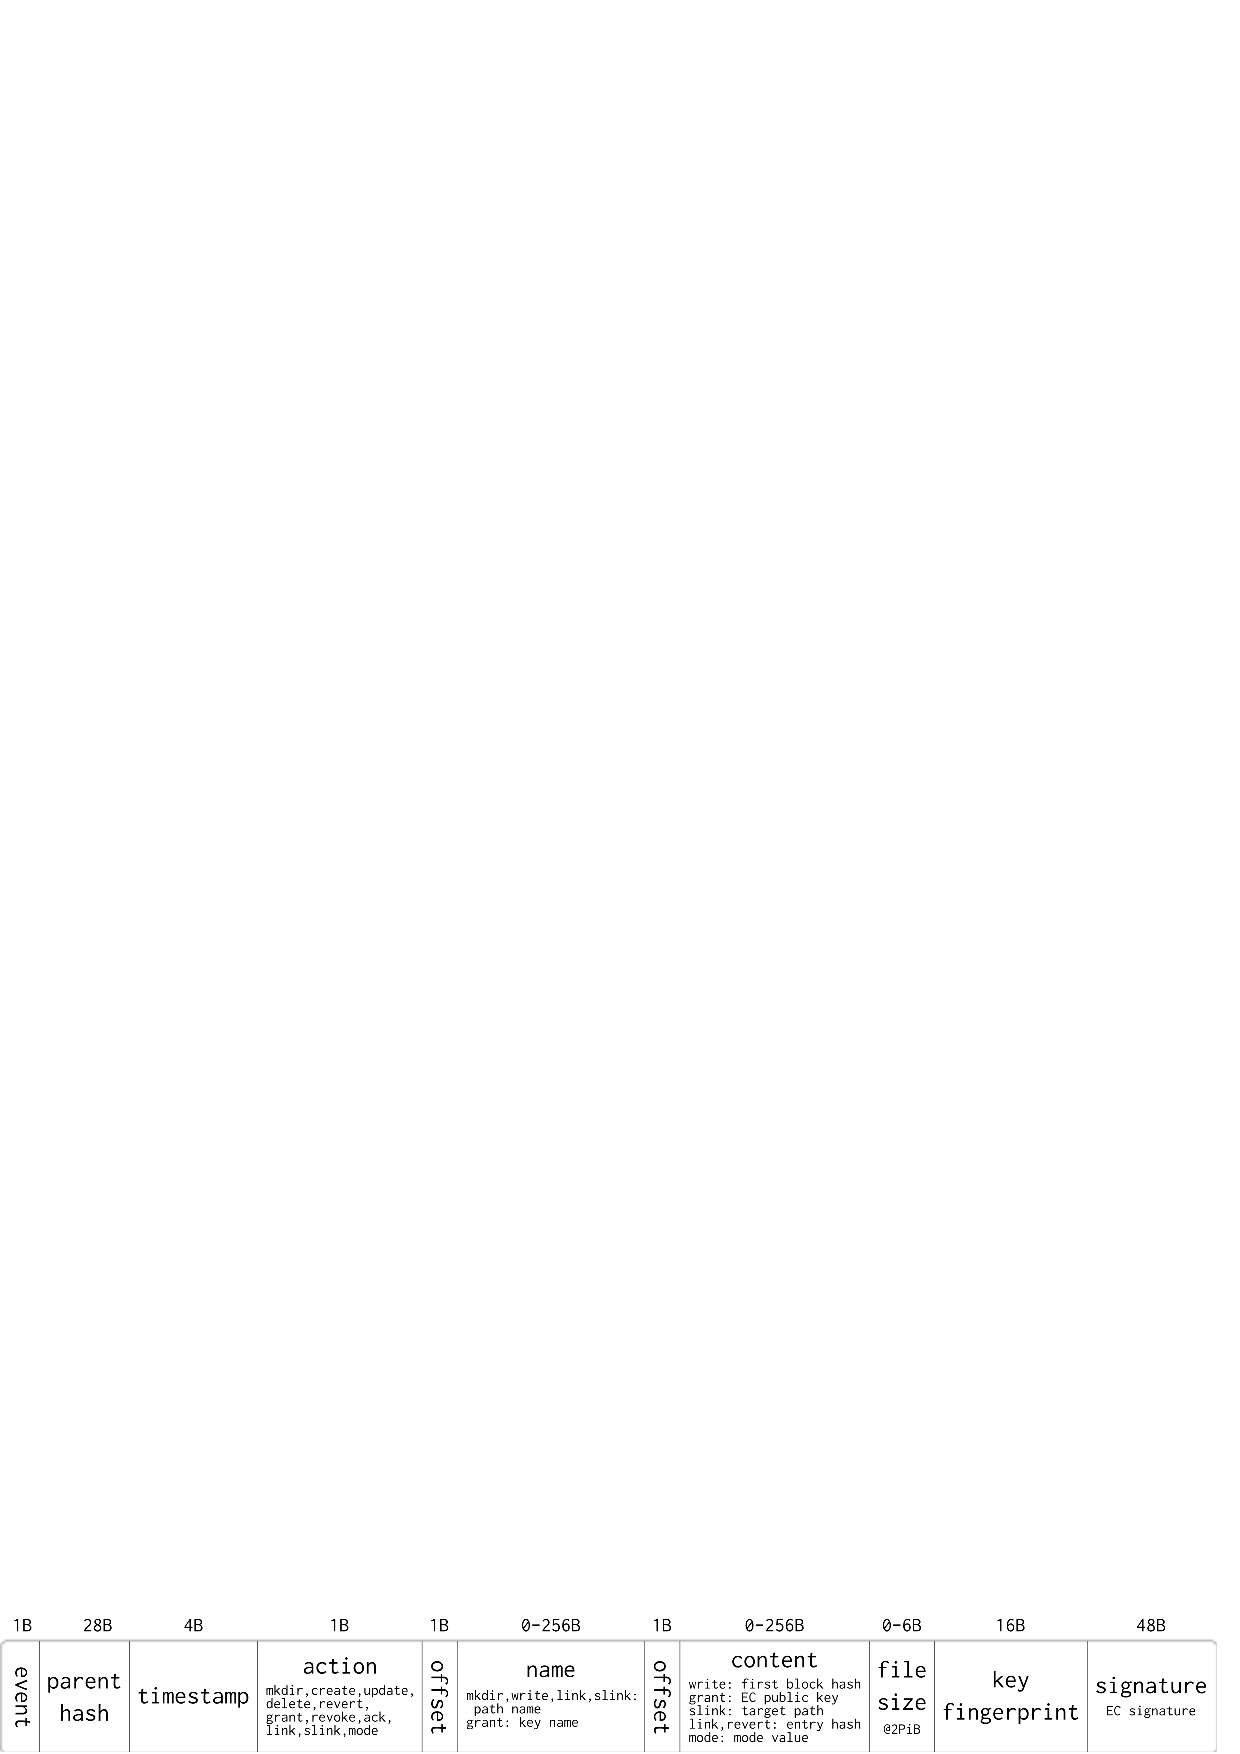
\includegraphics[width=\textwidth]{imgs/payload.png}
\caption{Log entry contained into a Serf custom event payload}
\label{fig:etc-time}
\end{figure*}


\begin{enumerate}
\item The hash function of choice is SHA-224, the smallest SHA (28B) considered secure\footnote{\url{https://en.wikipedia.org/wiki/SHA-2\#Comparison\_of\_SHA\_functions}}.
\item We use elliptic curve cryptography with 192bits key size (equivalent to a 2048b RSA key\footnote{\url{https://tools.ietf.org/html/draft-ietf-msec-mikey-ecc-03}}). Keys of this size produce  48 Bytes signatures.
\item File size value is limited to 6 bytes, restricting the maximum file size to 2 PiB.
\item Even though text protocols are easier to work with, we choose to use a more space-efficient binary representation of the entry fields. When possible, field delimitation is based on the field size. Otherwise, a dedicated offset byte is used, which can delimit up to 256byte, just enough to comply with our 256 character upper limit on names.
\end{enumerate}

Even though the efforts made compacting log entries, log blocks are another story. Updates uses bsdiff4 algorithm, which produces a very space-efficient binary diff of two files. Therefore, most of the updates will fit into a single Serf event. However, if updates are big they will not. Fortunately, configuration files are small. In order to have a better understanding of how many events are needed in worst-case scenarios we have characterize the \texttt{/etc} directory of a few Linux system, since all the results are very similar we only present the results of a web server running Debian in figure \ref{characterization}

full state sync disemination probability 1

\begin{figure}[htp]
\centering
\includegraphics[width=\columnwidth]{../eval/plots/etc_messages.png}
\caption{Cumulative histogram of /etc number of messages}
\label{fig:etc-messages}
\end{figure}

\begin{figure}[htp]
\centering
\includegraphics[width=\columnwidth]{../eval/plots/etc_time.png}
\caption{Compression time of /etc files}
\label{fig:etc-time}
\end{figure}


% todo characterization


They are used for maintaining cluster membership and for broadcasting short events to all the cluster members.

BaseFS uses Serf, a tool for cluster membership, failure detection, and orchestration that is decentralized, fault-tolerant and highly available.


cluster membership and event broadcast a gossip protocol

[1]http://citeseerx.ist.psu.edu/viewdoc/summary?doi=10.1.1.160.2604

a) cluster membership maintenance, b) failure detection and recovery of members and c) broadcast of short events to a cluster.



Gossip protocols, in general and serf in particular, have been useful for two tasks: membership maintenance and broadcast of short events (usually of the size of a UDP packet). The properties that enable:

\begin{itemize}
\item scale well in number of nodes, the number of messages stays constant as nodes are added. 
\item strong completeness of crashed-failing nodes
\item speed of failure detection
\item accuracy
\end{itemize}



re very efficient and accurate on maintaining cluster membership and detecting failling nodes.


\subsubsection{Synchronization Protocol}

While gossip produces the initial spread of information, a full state synchronization protocol is run infrequently in order to deal with nodes rejoining the cluster after being partitioned, or when a failed node is replaced or partially recovered. Additionally, because the number of blocks sent through the gossip layer is limited, a mechanism to spread remaining blocks is needed.

In order to make the information exchange during replica synchronization efficient, BaseFS uses Merkle trees. Data is hashed at multiple levels of granularity and nodes can quickly find out which part of the data is divergent. The Merkle tree is built conforming to the filesystem hierarchy. Each path hash is computed recursively, using the XOR of its sub-paths as well as its own related entries. The root path is the XOR of all the log entries. The protocol communication is an iterative process, walking and expanding those paths with a mismatching hash. Nodes will detect divergence and interchange log entries and blocks until they are fully synchronized.

The block hashes are not included on the Merkle tree. Doing so will make the synchronization protocol very unstable during periods of gossip dissemination. The root hash will flap its value very rapidly. To avoid this effect, as well as preventing nodes to simultaneously retrieve the same blocks from multiple peers, we introduce the notion of \textit{block state}. Files can be in one of the following three states:

\texttt{SEED\_NODES}

\begin{figure}[htp]
\centering
\includegraphics[width=170pt]{imgs/blockstate.png}
\caption{Block state diagram}
\label{fig:blockstate}
\end{figure}


\begin{itemize}
\item Receiving - indicates an initial state, the node has received a new \textit{write} entry. The sync protocol will announce this file as being received, no change performed to the Merkle tree.
\item Stalled - a file enters this state when no related block has been received after some time $t$. Both, the entry hash and the last received block are added to the Merkle tree.
\item Completed - all related blocks have been received. The \textit{Entry} hash is included to the Merkle tree. In case the previous state was stalled, the last block hash is removed.
\end{itemize}


The synchronization protocol is a text-based streaming protocol, using new line characters as delimiters and encoding binary information (block content) in base64. Its alphabet is:

\begin{itemize}
\item \texttt{HASH} - Filesystem root hash. Only sync when equal TODO REPHRASE
\item \texttt{LS} - Path list, includes all path entry hashes, sub-paths hashes and the last-block hash of incomplete files.
\item \texttt{PATH\_REQ} - Path request, indicates a node is missing an entire path and requests all its content to its peer.
\item \texttt{ENTRY\_REQ} - Entry request, used by a node to request a missing entry to its peer.
\item \texttt{BLOCK\_REQ} - idem for blocks
\item \texttt{ENTRIES} - Contains a log entry, can be a response to an \texttt{ENTRY\_REQ} or when a node finds out that its peer is missing some entry.
\item \texttt{BLOCKS} - idem for blocks
\item \texttt{BLOCKS\_REC} - A node announces files in receiving state. In case of divergence the peer can apply this hash to the Merkle tree.
\item \texttt{CLOSE} - Indicates a node is fully synchronize with its peer and communication is terminated.
\item \texttt{EOF} - End of transmission. TODO
\end{itemize}


The pattern of communication is probabilistic, nodes have some probability $p$ of attempting to synchronize with each other. Every $t$ seconds, each node picks a node to communicate with. To initiate synchronization nodes send a \texttt{HASH} and \texttt{LS /} requests containing their own state, and things continue from there.



\section{BaseFS Implementation}

\begin{itemize}
  \item \textbf{Filesystem} - The emulation of filesystem operations on \textit{view} operations. Described in \ref{filesystem}.
\end{itemize}


\begin{figure}[htp]
\centering
\includegraphics[width=\columnwidth]{imgs/modules.png}
\caption{BaseFS modules}
\label{fig:modules}
\end{figure}


BaseFS makes extensive use of concurrency including processes, threads and an event loop. The FUSE interface runs on the main Python thread, as required by its implementation. The Serf agent runs on a separated Python process, and we talk with it using Serf own RPC protocol. We spawn an additional thread for the event loop. Implemented with asyncio, the event loop handles all the remaining network communication in a non-blocking fashion, including the sync protocol, receiving of custom gossip events and commands sent by BaseFS CLI utility. The event loop thread shares memory with the main FUSE thread, and only a single instance of the View has to be maintained, saving memory and computation time.

File Handler also spawns a new process for each registered handler script

\subsection{Filesystem}
The filesystem layer is implemented using FUSE Python bindings\footnote{\url{https://github.com/terencehonles/fusepy}}. FUSE stands for Filesystem in Userspace, and Wikipedia defines it as "an operating system mechanism for Unix-like computer operating systems that lets non-privileged users create their own filesystems without editing kernel code". This is achieved by running filesystem code in user space while the FUSE module provides only a "bridge" to the actual kernel interfaces. The implementation is very straightforward, and almost limited to \textit{View} operations.


The filesystem, however, needs to be aware of new changes made by other nodes. Because of its cost, the \textit{view layer} does not rebuild automatically when new changes arrive. Instead each time we want to read something, the filesystem layer checks if its log seek value is up-to-date with the actual log seek value. A mismatch indicates new entries have arrive and a rebuild of the \textit{view} is performed before doing the actual read.

Another detail worth mentioning is the caching layer used for file write operations. Because the blabla we cluster writes so we can do diff, and safe staff

\subsubsection{Watchers}
The naive approach for applications to react to changes is periodic reading (pulling) the state they are interested in. Modern Linux kernels provide support for filesystem notifications via the inotify subsystem. Unfortunately FUSE is missing support for triggering those events. Since the main objective of BaseFS is to act as a middleware providing shared state between applications, contribute and effective mechanisms that allow applications to react to state changes is very convenient. Support for executing scripts in response to new log entries is natively provided in the form of event handlers.

Event handlers are registered on mounting time and can be any executable, including piped executables (such as \texttt{awk '{print \$2}' | grep foo}), since event handlers are invoked within the context of a shell. The event handler is executed anytime a new log entry is stored. Context for the scripts is given by \texttt{BASEFS\_EVENT\_TYPE} and \texttt{BASEFS\_EVENT\_PATH} environment variables. 


\subsection{Commands}

order by step to get sense of how to proceed, get service discovery with DNS TXT records

\begin{itemize}
 \item mount	Mount an existing filesystem
 \item run		Run an existing filesystem without mounting it (testing)
 \item bootstrap	Create a new self-contained filesystem
 \item genkey	Generate a new EC private key
 \item keys	List keys and their directories
 \item grant	Grant key write permission
 \item revoke	Revoke key write permission
 \item list	List all available logs
 \item show	Show a log file using a tree representation
 \item revert	Revert object to previous state, 'log' command lists all revisions
 \item blocks	Block state
 \item members	List cluster members
 \item serf	Serf RPC Command proxy
 \item get		Get log from peer address
 \item installserf	Download and install Serf
 \item resources	Display BaseFS resource consumption in real-time
\end{itemize}


\section{BaseFS Evaluation}



In this section we present an evaluation of the BaseFS network properties and IO performance. For the validation of the Merkle DAG conflict resolution and permissions the reader can refere to the unit and functional tests shiped with BaseFS source code\footnote{\url{https://github.com/glic3rinu/basefs/}}.

All test scenarios have been fully automated for easily reproducability. We have developed our own test suit. The test suite has support for virtual environments based on Docker containers and TC, as well as support for Community-Lab testbed. Docker builds on top of the Linux kernel resource isolation features to provide operating-system-level virtualization. On the other hand, TC (Linux Traffic Control), is a shell utility that can be used for configuring the kernel network scheduler and shape the traffic characteristics at will, like packet loss and delay. Community-Lab is Community Netwotk Testbed by the CONFINE project that provides a global facility for experimentation with network technologies and services for community networks. Support for deploying, orchestrating and collecting experimental data on Community-Lab is provided by utilities written in Bash and Python, using concurrent multiplexed SSH sessions underneeth.

It is also worth mentioning that BaseFS has a built-in profiler that keeps track of resource usage and other metrics like memory, CPU, network usage or context switches.

During the execution of experiments the test suit will tear up and down hundreds of Docker containers, particularly on scalability tests. To avoid an ARP table overflow the system \texttt{net.ipv4.neigh.default.gc\_thresh3} has to be increased. We found 32768 to be a sane value. https://github.com/hashicorp/serf/issues/263

\subsection{Network Evaluation}
The network evaluation is separated into three main phases. The first two are independent evaluations of the gossip layer and the sync protocol on a virtual environment using Docker and TC. By shaping the traffic we are able to see how differnet network conditions affect the convergence characteristics and traffic usage of both protocols. With that information we will move to the next phase and make an informed decission about the prefered values for \texttt{MAX\_BLOCK\_MESSAGES} and \texttt{FULL\_SYNC\_INTERVAL}. Then we will evaluate the behaviour of both protocols working togerther. In this phase, BaseFS will be additionally tested on Community-Lab.

Each experiment is performed on a cluster of 30 nodes. For each experiment a new BaseFS log is bootstraped. Nodes get and mount this freshly created BaseFS filesystem. The cluster members are given a few seconds to find each other. We simulate configuration updates by copying a set of pre-created files into one of the nodes BaseFS mounted partition. Then we meassure the time it takes for the configuration file to propagate to the rest of the cluster. The test files have different sizes but they are always the same on all experiments, so the results are comparable. We monitor the number of converged nodes in real time, so the experiment can advance as soon as all nodes have received the updates. We define a maximum waitting time of 100 minutes between file copies, with an additional maximum of 150 minuts at the end of each experiment.


\paragraph{Max gossiped messages}

For the gossip layer experiments we have disabled BaseFS sync protocol and configured \texttt{MAX\_BLOCK\_MESSAGES} to an arbitrary large number, enssuring that the only communications between BaseFS nodes will be by means of the gossip layer. We will see how network conditions like delay, packet loss, packet reordering or bandwith limitations affects the convergence time of the cluster. We define convergence as te time required for a log entry, and its related blocks, to spread over the entire cluster.


\begin{figure}[htp]
\centering
\includegraphics[width=\columnwidth]{../eval/plots/gossip.png}
\caption{Gossip convergence with variable number of gossip messages}
\label{fig:gossip}
\end{figure}

\paragraph{Fullsync Interval}

The key characteristic for the sync protocol is how the synchronization interval affects the convergence time and traffic usage of the synchronization protocol

\begin{figure}[htp]
\centering
\includegraphics[width=\columnwidth]{../eval/plots/sync.png}
\caption{Full Sync protocol convergence with variable execution interval}
\label{fig:sync}
\end{figure}



Define a realistic scenario, tune the \texttt{MAX\_BLOCK\_MESSAGES} and \texttt{FULL\_SYNC\_INTERVAL} to a reasonable values.


\paragraph{Scalability}

\begin{figure}[htp]
\centering
\includegraphics[width=\columnwidth]{../eval/plots/scalability.png}
\caption{BaseFS Docker scalability}
\label{fig:scalability}
\end{figure}

Since our machine has 4 cores, everything beyond a load of 4 should be considered overload. CPU contention

our system has a total of 7688200K which and each basefs process consumes arround 2400 KB of resident memory we should hit swap at arround 300nodes ($7688200/24200$)

also serf simulator \footnote{https://www.serfdom.io/docs/internals/simulator.html} 2.7 seconds 99.975\% for 290 nodes, and we observe a convergence time of arround 11 seconds.

so if we want to to get consistent results we have to maintain the number of nodes of our experiments below 50, and since we will be using the machine while the experiments are running, we will be conservative and keep the experiments limited to 30 nodes.


Now we study the BaseFS behaviour, gossip and sync protocols working in tandem in two different envirnoments. First using a simulated perfect environment using Docker, and then we replicate the experiment on COnfine testbed.

The generated workload consists of 560 writes separated by 3 seconds. The writes are crafted in order to generate predetermined amount of gossip packets, simulating a workload typical configuration management operations. We have erred on the side of more packets than those we believe will be acctually needed on real scenario, since configuration updates usually involves a really small amount of data that can easily fit into a single gossip message.

0: 340 0.60 1: 160 0.28 2: 20 0.03 4: 20 0.03 16: 20 0.03 total: 560 writes


\subsubsection{Delay Effects}

TC netem discipline provides network emulation functionality for testing protocols by emulating the properties of wide area networks. In this section we will see how the gossip layer, or Serf for that matter, is affected by packet delay. Typically, the delay in a network is not uniform. It is more common to use a something like a normal distribution to describe the variation in delay. We have created multiple distributions with different mean, and a designated standard deviation of 20\% of the mean value on each case. \texttt{netem delay 100ms 20ms distribution normal}


\begin{figure}[htp]
\centering
\includegraphics[width=\columnwidth]{../eval/plots/basefs-delay.png}
\caption{BaseFS under variable delay}
\label{fig:basefs-delay}
\end{figure}


Serf is configured to use the WAN profile with a ProbeTimeout of about 3 seconds. This is important because under network latency greater than 3 seconds nodes will be reported as failed. In this experiment, Serf failure detector mechanism show its robustnes. Because of the delay normal distribution, some packets will still get lower than 3 seconds delays, andvalues messages will not spread and the protocol will not converge. This is further confirmed by looked at Serf debugging messages, we start to get some \texttt{Marking 0242ac110014-8ab678bdbfa1 as failed}, suspect timeout reached from delay mean starting from 1280ms.

How relevant latency is in the context of Community Networks? DOes long distance wireless links add lots of it? is bufferbloat worth mentioning since UDP is not that much affected?

this is where the limitations of the gossip protocol start to show up

Serf perform surprisingly well under very large delays.



\subsubsection{Packet Loss Effects}

In this section we evaluate the packet loos effects on the gossip layer. We have used the netem module to simulate various degrees of packet loss. In real networks, packets are lost in bursts, with a non independent probability. Netem allows to specify a correlation value and simulate packet loss episodes. \texttt{netem loss 30\% 25\%} will cause 30\% of packets to be lost, and each successive probability depends by a quarter on the last one.

$P_n = .25 * P_n-1 + .75 * Random$

For our test we have evaluated packet loss in increments of 10\% and a constant correlation of 25\%. Figure 2 shows de results of such experiments. Figure 3 shows the \% of convergence reached on each scenario.

\begin{figure}[htp]
\centering
\includegraphics[width=\columnwidth]{../eval/plots/basefs-loss.png}
\caption{BaseFS under variable packet loss}
\label{fig:basefs-loss}
\end{figure}

For understanding the results, we need to know that Serf WAN profile is configured with GossipNodes of 4 nodes, meaning that nodes will gossip a message to another 4 random peers. Because gossip messages are transported over UDP, without acknowledgment of received data, heavy packet loss has a large impact on the convergence time. To mitigate this effect Serf runs a second protocol for performing periodic full state synchronization. But still, Figure 2 shows how intense packet loss prevents the cluster from converging. Looking at the Serf debug logs, collected during the experiment, we can make two educated guesses about the reasos why. First, it may be because members are continually reported as failed and peers do not attempt to contact them. Second, Serf event queue has a limit of messages it can hold, this may have a cumulative effect and earlier messages are lost before the full state sync can have a chance to work its magic. In any case, packet loss up to 20\% does not seem to have a significative effect, up to 50\% of packet loss the protocol can converge on all scenarios. Things get ugly at 80\% of packet loss, but under that conditions the entire network would be rendered usseless anyway.

\subsubsection{Packet Reordering Effects}
Packet reordering or out-of-order delivery is the delivery of data packets in a different order from which they were sent. Out-of-order delivery can be caused by packets following multiple paths through a network. Netem can simulate reordering, with correlation, in a similar way as how packet loss is specified \texttt{netem reorder 50\% 25\%}.


\begin{figure}[htp]
\centering
\includegraphics[width=\columnwidth]{../eval/plots/basefs-reorder.png}
\caption{BaseFS under variable packet reordering}
\label{fig:basefs-reorder}
\end{figure}

Packet reordering happens naturally during the execution of a gossip protocol; nodes are expected to receive messages from different nodes at different order. This is why no matter how sever it is, our simulated packet reordering has no effect whatsoever on the convergence time of the gossip layer.

\subsubsection{Bandwith Limitations Effects}

For rate control we use Hierarchical Token Buckets (HTB) queueing dicipline that allows to define link data rates as easy as \texttt{htb rate 32kbit}. It is true that on wireless networks link speed may be something very dynamic under acute interference. However, we will not simulate dynamic

The results are consistent from what is expected from Serf. Using the simulator with WAN parameters Gossip Fanout of 4, Gossip Interval of 0.5 seconds and a number of 30 nodes, we get an estimated max bandwidth: 175 kbps/node

Received event: member-failed Suspect 0242ac110012-e98725c7c319 has failed, no acks received

TODO repeate 56 32kbps give it more time for final convergion. Serf gossip protocol behaves decently under high constrained bandwith conditions. It is not until we reduce the traffic to 56kbps and generate a burst of 100 messages

There is no rate control built-in to the netem discipline, instead use one of the other disciplines that does do rate control. In this example, we use Token Bucket Filter (TBF) to limit output. 50 packets buffer (seems to be the deafult, 75000bytes, )

\begin{itemize}
 \item burst, also known as buffer or maxburst. Size of the bucket, in bytes. This is the maximum amount of bytes that tokens can be available for instantaneously. In general, larger shaping rates require a larger buffer. For 10mbit/s on Intel, you need at least 10kbyte buffer if you want to reach your configured rate! https://en.wikipedia.org/wiki/Token\_bucket
 \item limit or latency Limit is the number of bytes that can be queued waiting for tokens to become available. latency parameter, which specifies the maximum amount of time a packet can sit in the TBF 
\end{itemize}

\begin{figure}[htp]
\centering
\includegraphics[width=\columnwidth]{../eval/plots/basefs-bw.png}
\caption{BaseFS under variable bandwidth}
\label{fig:basefs-bw}
\end{figure}


\subsubsection{BaseFS Under CommunityLab}

We have deployed BaseFS over CommunityLab testbed and meassure the convergence time of a simulated workload. We replicated the same experiment using Docker containers, so we can compare the results with a more idealistic scenario.

In order to use the testbed we have created an slice with all available nodes in \textit{production} state and with support for public IPv4 addresses (from the context of CN). Because some of the nodes (slivers, in CONFINE terminology) did not have Internet connection we deployed our own APT (Debian package manager) and PIP (Python package manager) proxies, so we could install the BaseFS required dependencies in all slivers. Also, NTP traffic for slivers is filtered, so we also deployed our own NTP (Network Time Protocol) on the management network \footnote{https://wiki.confine-project.eu/arch:management-network} to ensure all sliver's clocks are properly synchronized for our experiments. 



\paragraph{Docker}

Controlled Virtual environment with Docker and TC * Each node runs on a Debian 6 Docker container with a virtual ethernet device. Nodes are connected with one level 2 hop between them. This is a controlled environment and we use Linux traffic control to emulate variable delay, packet loos, duplication and re-ordering, in order to understand its effects on BaseFS's communication protocols.

\paragraph{CommunityLab Testbed}

Ralistic environment on Confine testbed * Each BaseFS node runs on a Debian LXC container on top of a Confine Node. Confine Nodes are heterogeneous devices and resources are share with other ongoing experiments, which makes for a very inconsistent performance characteristics. All our nodes are connected using the native IP network provided by different community networks where Confine nodes are deployed. Since we don't have much control of the underlying infraestructure we provide a network characterization to better understand the environment where the experiment is taking place.

Network characterization

Because we run the experiment on a pre-existing and not configurable network topology we need to characterize and discover the propertires of the network to have a better understanding of the experimental results.


\begin{figure}[htp]
\centering
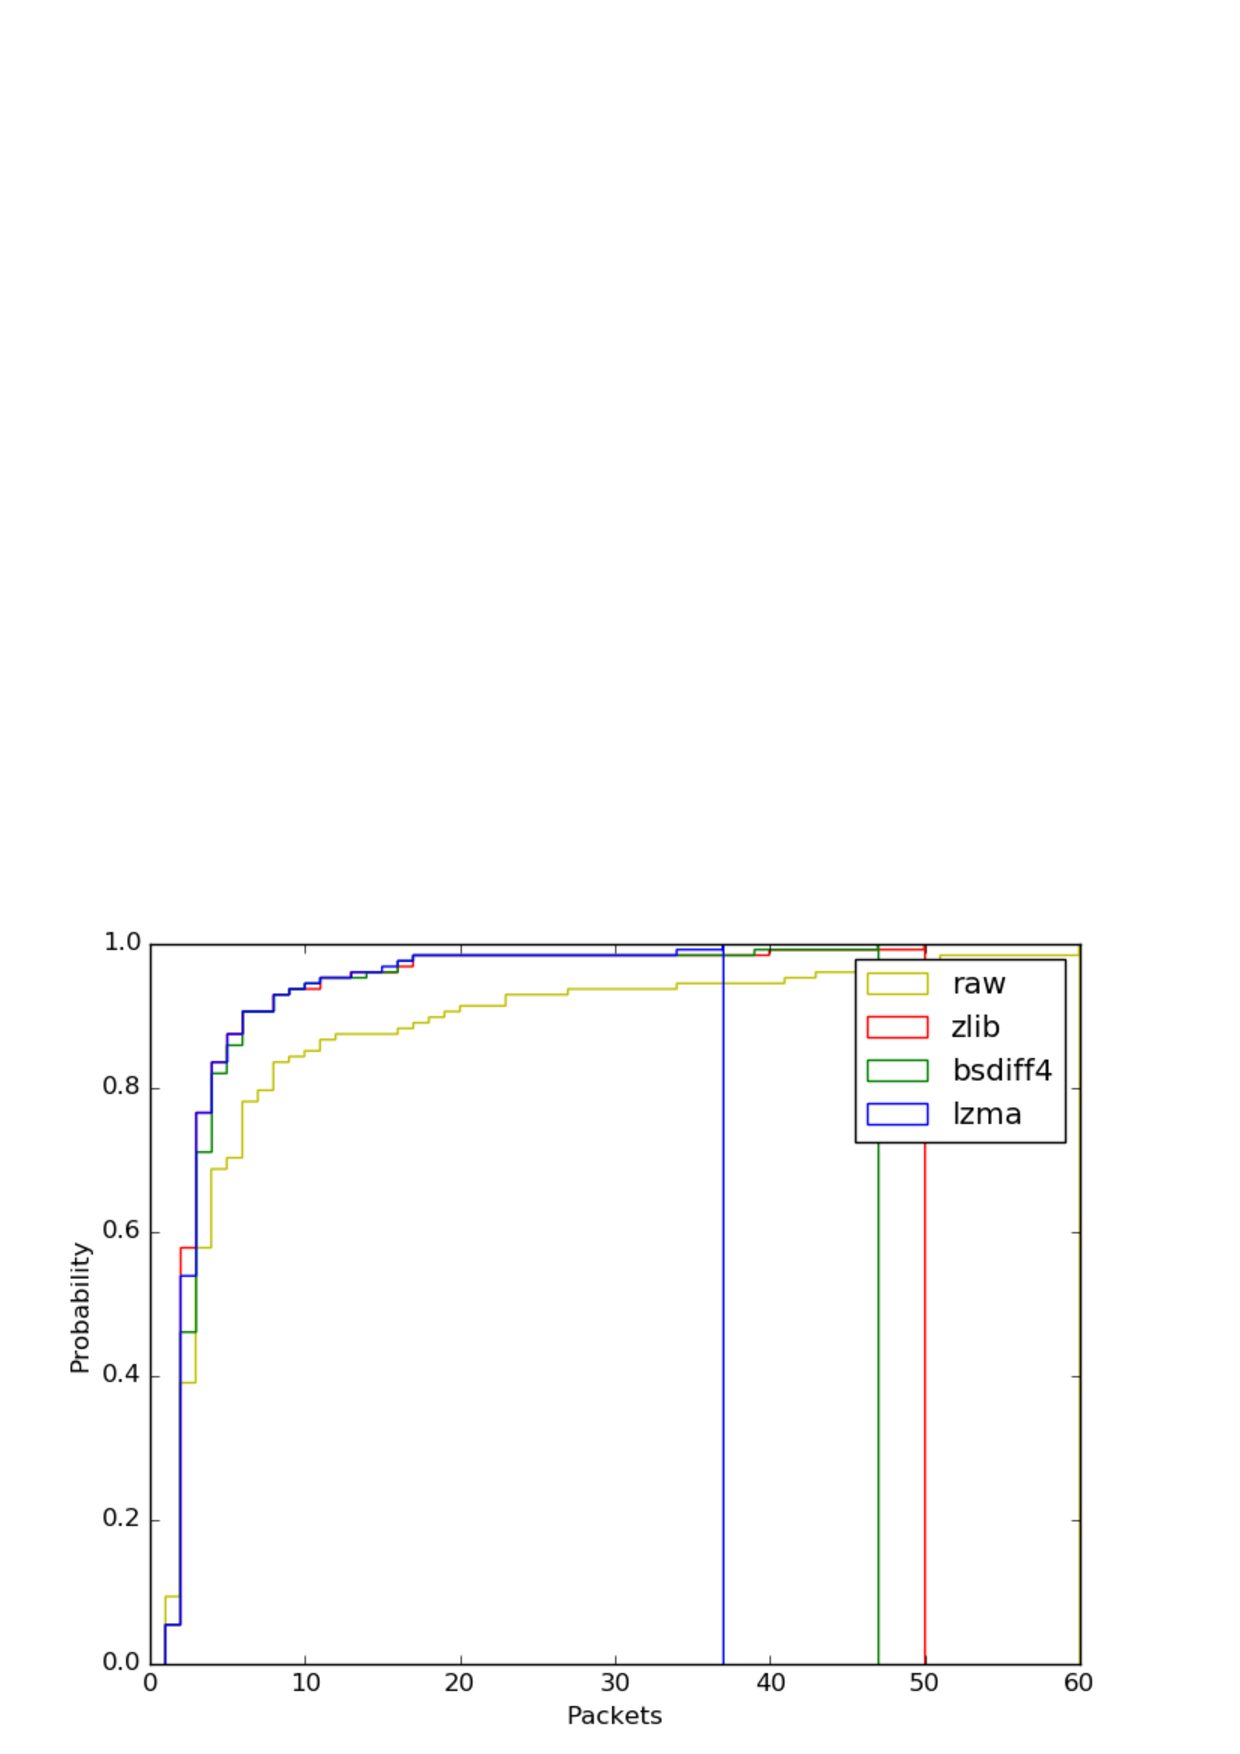
\includegraphics[width=\columnwidth]{../eval/plots/characterization.png}
\caption{CommunityLab network hops}
\label{fig:characterization}
\end{figure}

\begin{figure}[htp]
\centering
\includegraphics[width=200pt]{imgs/topology.png}
\caption{CommunityLab network topology}
\label{fig:topology}
\end{figure}

gossip layer saturation limit
etc characterization
    bsdiff (designed for executables) ram hungry: bsdiff is quite memory-hungry. It requires max(17*n,9*n+m)+O(1) bytes of memory, where n is the size of the old file and m is the size of the new file. bspatch requires n+m+O(1) bytes.



\begin{figure}[htp]
\centering
\includegraphics[width=\columnwidth]{../eval/plots/basefs.png}
\caption{BaseFS convergence time on CommunityLab}
\label{fig:basefs}
\end{figure}

\begin{figure}[htp]
\centering
\includegraphics[width=\columnwidth]{../eval/plots/basefs-traffic-distribution.png}
\caption{BaseFS traffic distribution on CommunityLab}
\label{fig:basefs-traffic-distribution}
\end{figure}

Even though we didn't intend to have nodes behind NAT for this experiment, we found that there was a problem requesting public IP addresses, and node 9 and 29 where placed behind a NAT. This means that contact initiatied by other nodes was not possible, but they still can recieve log entries by means of the sync protocol. We have validated that BaseFS can work even behind a NAT and a few nodes do not appear to have a significant impact on its performance.


\subsection{File Operations Performance}
    
In this secction we compare BaseFS to a more traditional file system (EXT4). We made the experiments to roughly show how file updates affect read and write performance at the filesystem level, while having a known filesystem to help putting results into prespective. The experiemnt consists on copying up to 30 times the entire content of the \texttt{/etc} root directoy (files, directories and simbolic links), simulating a worst case write workload that we can expect from a configuration managemnet utility.

The \texttt{/etc} directory of the testing machine contained

\begin{itemize}
 \item 2512 files
 \item 1350 symbolic links
 \item 462 directories
 \item 22 MB of data
\end{itemize}
Bear in mind that we are comparing a kernelspace filesystem (EXT4) with a userspace virtual filesystem that requires executing complex algorithms on top of cPyhton, with the additional FUSE layer and the added cost of having to context switch into kernel mode for performing system calls.

\subsubsection{Read Performance}

Starting from a fresh log file, on each round we recursively copy the entire \texttt{/etc} directory into BaseFS mounted directory. Then we perform two reads, the first needs to compute the binary difference of every previous version, but the second is cached. We do the same with an EXT4 filesystem stored on a SATA drive. In this case, however, we perform a \texttt{sync \&\& echo 3 > /proc/sys/vm/drop\_caches} after every write i order to clean any possible caching and do the first read as cold as the BaseFS one.

\begin{figure}[htp]
\centering
\includegraphics[width=\columnwidth]{../eval/plots/read_performance.png}
\caption{BaseFS vs EXT4 filesystem read performance}
\label{fig:read-performance}
\end{figure}

As expected, cold read performance is linearly affected by the incresing number of patches requiered to apply for obtaining the most recet version of the content of each configuration file. However, a cached BaseFS reads are faster than uncached EXT4 reads, being able to read the entire filesystem clocking at about 2 seconds.

\subsubsection{Write Performance}


Figure 10 shows how BaseFS write performance compares to EXT4. We can see how in each additional recursive copy of the \texttt{/etc} directory into the BaseFS partition increases the cost consistently. Apart from writing to the log file, BaseFS calculates the binary difference of each file and computes the conflict-free view of the filesystem. Sure, this process can be greatly optimized, however we should not be really concern about the performance of massive write operations, since cluster configuration is about changing small bits of information, and we have already demonstrated the subsecond convergence properties of BaseFS


\begin{figure}[htp]
\centering
\includegraphics[width=\columnwidth]{../eval/plots/write_performance.png}
\caption{BaseFS vs EXT4 filesystem write performance}
\label{fig:write-performance}
\end{figure}

Cache invalidation is a hard problem to takle and is effectively limiting what we are able to cache without paying a great cost on implementation complexity. For one, the conflict-free view of the entire filesystem is recomputed on reads that come after writes. On the other hand, the file content is also invalidated on a write operation and the binary difference has to be computed using all the BSDIFF4 patches that have been generated since file creation, increassing the cost on each update.

We have made the choice of using BSDIFF4 binary deltas on the grounds that write-intensive workloads are not expected for a cluster configuration tool and a faster convergence time (less messages to gossip) is a more desirable characteristic.

In order to understand the read and write perfomance characteristics we compare BaseFS with a more traditional and popular file system (EXT4). This experiment shows how file updates affects read/write completion time.

Cluster configuration does not need to hold up to high intensive IO workloads, a faster convergence time is a more interessting property. However, BaseFS does remarkably well, even though it has not been finely tuned for filesystem IO performance.

BaseFS makes extensive use of concurrency including processes, threads and an event loop. The FUSE interface runs on the main Python thread, as required by its implementation. The Serf agent runs on a separated Python process, and we talk with it using Serf own RPC protocol. We spawn an additional thread for the event loop. Implemented with asyncio, the event loop handles all the reamaining network communication in a non-blocking fashion, including the sync protocol, receiving of custom gossip events and commands sent by BaseFS CLI utility. The event loop thread shares memory with the main FUSE thread, and only a single instance of the View has to be maintained, saving memory and computation time.



\section{The Future}

Generalized filesystem better support for big files should be in order: Incentives, bt swarm, infohashes, multiple block encoding

block encription for read permissions

locality aware sync protocol based on serf coordinates

infohash expands manifest until address space is big enough to fit all the file block hashes

Some nice features have been left out of the scope of this project, just because our focus has been to proof that our idea works and has meaningful value.

Multiple diff algorithms for diffing, maybe let user choose.
diff of large files, don't put them in memory: fs mount option?

Node certificiate to make sure we GET logfile from the correct device and not some rouge node
\begin{figure}[htp]
\centering
\includegraphics[width=\columnwidth]{imgs/infohash.png}
\caption{Alternative block linking with manifest tree}
\label{fig:infohash}
\end{figure}


enabler for decentralizate cloud platforms

provide plugable block algo, instead of desiding what works best for each use case 
gossip layer problems: Keep track of bad behaviour and ban bad nodes.

sync protocol room for imporvement: biased instead of rand uniformly distributed
For small files it is not really important to give incentives for sharing because the resources that each node has to contribute for becoming part of the network are small. However for large files or very-very large file systemes we can consider to incentive mechanisms:
    a) block-market swarn: write content contains all the blocks hashes of that file, the original content has to be fetched from a bitTorrent-like swarm, much like swaptorrent works (ipfs)
    b) nodes do not contribute all the missing parts when syncing, they can keep track of the behaviour of the other nodes and decide to choke them if appropiate

more than cluster management

a. decentralized state
    Dropbox-like applications: each user with each folder, and shared folders
    SO upgrade on large clusters
    shared configuration for decentralized cloud computing: zookeeper, etcd
    shared in-memory-state for clusters: memcached

b. mutable P2P content
    Mutable P2P file sharing, ok for small files, but incentive mechanissm to avoid free-riders and block sharing swarm may be needed (WRITE magnetlink).
    Live documents: enciclopedia or discographies that self-update when new updates are available

c. monotonicity
    Version control system

Notice that file contents nor metadata (size, name, date) are not encrypted in anyway. Privacy is left intentionally out of the scope of this project since our focus is to prove that our idea works. 


Biased getPeer(randomize algorithm) : network proximity, published new content
imporve serf membership maintenance: when a failing node is remove from the member list?
If baUery power, bandwidth, and other resources are scarce, selfish users may not wish to forward packets for other users
\section{Conclusions}

we presented a system with properties that enables more than decentralize configuration.%\end{document}  % This is where a 'short' article might terminate


\section{Acknowledgments}
The authors would like to thank Ester Lopez for her help in providing most of the \texttt{R} code for the plots contained in this document.

%
% The following two commands are all you need in the
% initial runs of your .tex file to
% produce the bibliography for the citations in your paper.
\bibliographystyle{abbrv}
\bibliography{sigproc}  % sigproc.bib is the name of the Bibliography in this case
% You must have a proper ".bib" file
%  and remember to run:
% latex bibtex latex latex
% to resolve all references
%
% ACM needs 'a single self-contained file'!
%
%APPENDICES are optional
%\balancecolumns
%\balancecolumns % GM June 2007
% That's all folks!
\end{document}
